\documentclass[12pt,a4paper]{article}
\usepackage[utf8]{inputenc}
\usepackage{graphicx}
\graphicspath{{../Images/}}
\usepackage{amsmath}
\usepackage{amsfonts}
\usepackage{amssymb}
\usepackage{hyperref}
\usepackage[margin=1in]{geometry}
\usepackage{subfig}
\usepackage{float}
\usepackage{xcolor}
\hypersetup{
    linktoc=all,     %set to all if you want both sections and subsections linked
    linkcolor=blue,  %choose some color if you want links to stand out
}

\author{Thibaut Marmey}

\title{Notes de cours C}
\begin{document}
	\maketitle
	
\begin{normalsize}
\tableofcontents
\end{normalsize}

\section{Bases}
\subsection{Général}
\begin{itemize}
\item \textbf{int main(int argc, char **argv)} : \textit{argc} représente le nombre d'arguments lors de l'exécution du programmes. Sans aucun argument \textit{argc = 1}.
\textit{**argv} représente quand à lui la liste des arguments déclarés lors de l'exécution du programme.
\item Si l'on veut passer un int en paramètre du programme, utliser : \textit{atoi(argv[indice])}
\newline Cela permet de convertir le \textit{char} récupéré comme paramètre en \textit{int}.
\item Taille des différents types de données
\newline
\begin{tabular}{|l|c|r|}
  \hline
  type & size & value range \\
  \hline \hline
  char & 1 byte & -128 to 127 or 0 to 255 \\ \hline
  unsigned char & 1 byte & 0 to 255 \\ \hline
  signed char & 1 byte & -128 to 127 \\ \hline
  int & 2 or 4 bytes & -32,768 to 32,767 or ... \\ \hline
  unsigned int & 2 or 4 bytes & 0 to 65,535 or ... \\ \hline
  short & 2 bytes & -32,768 to 32,767 \\ \hline
  unsigned short & 2 bytes & 0 to 65,535 \\ \hline
  long & 4 bytes & ... \\ \hline
  unsigned long & 4 bytes & ... \\ \hline
  double & 8 bytes & ... \\ \hline
\end{tabular}
\item La condition \textit{if} est \textit{True} si la condition est différente de 0. 
\newline Ainsi si l'on a \textit{if(1/10)} la condition est \textit{False}. \textit{Explication : }1 et 10 sont deux int, le résultat est de 1/10 est 0.1 mais le résultat est aussi un int donc la troncature du int donne 0.
\newline \textit{if(-1)} est quant à lui \textit{True} car -1 est différent de 0.
\end{itemize}


\subsection{Les structures}
\begin{itemize}
\item typedef struct à expliquer
\item Calculer la taille d'une structure : sizeof(structure) \textbf{!=} sum sizeof(elements)
\newline Il y a un allignement de mémoire c'est à dire que comme le processeur lit des mots de 4 octets il rajoute des bits dits de "bourrage". Ainsi il faut calculer la taille d'une structure en multiple de 4.
\newline Il faut donc calculer la somme des sizeof(elements) et arrondir le résultat au multiple de 4 supérieur. \textit{ex : si la somme des sizeof est égal à 14 la taille de la structure est : sizeof(structure) = 16 octets}
\end{itemize}


\subsection{Pointeur}
\begin{itemize}
\item \href{http://www.cplusplus.com/doc/tutorial/pointers/}{\textbf{\textit{lien internet : }doc cplusplus.com sur les pointeurs}}
\item \textbf{Déclaration d'un pointeur} : la valeur d'un pointeur est une adresse. 
Initialisation à NULL.
Où s'il pointe sur une variable : int *ptr = \&var
ou int var = 1; int *ptr = NULL; ptr = \&var;
\item \textbf{Changer valeur d'une variable via pointeur : } int a = 1; int *ptr = \&var; *ptr = 2; La variable a est alors égale à 2;
\item Si ptr est un pointeur pointant sur a = 1. *ptr est la valeur de a.
\item \begin{tabular}{|l|c|r|}
  \hline
  objet & valeur & adresse \\
  \hline \hline
  i & 3 & AAAAA \\ \hline
  p (pointeur sur i) & AAAAA & CCCCC \\ \hline
  *p & 3 & AAAAA \\ \hline
  pp (pointeur sur p) & CCCCC & DDDDD \\ \hline
  *pp & AAAAA & CCCCC \\ \hline
  **pp & 3 & AAAAA \\ \hline
\end{tabular}
\item Créer un pointeur et lui donner seulement la possibilité de lire une variable et non la modifier : \textit{const} int *p = \&a
\item void pointers est un pointeur qui n'a pas de type associé. Il peut prendre tout type de variable (le cas de malloc() ou calloc()). Dans un printf par exemple, le void pointer ptr doit être caster \textit{ex : printf("\%d", *ptr)} ne marche pas. L'expression \textit{printf("\%d", *(int *)ptr)} quant à elle marche.
\item Pointeur d'une fonction généralement pour passer une fonction en argument d'une autre fonction. \textit{ex : }
\newline int operation (int x, int y, int (*functocall)(int,int)) \{
\newline int g;
\newline g = (*functocall)(x,y);
\newline return (g); \}
\newline pour l'utiliser : m = operation (7, 5, addition);
\newline int (*minus)(int,int) = subtraction; \textit{permet de créer un pointeur de fonction qui prend deux int en argument}
\newline n = operation (20, m, minus);
\end{itemize}

\subsection{Fonctions}
\begin{itemize}
\item \href{https://www.codingunit.com/c-tutorial-the-functions-malloc-and-free}{\textit{lien internet : }utilisation de malloc}
\newline Utiliser \textit{int *ptr = (int *)malloc(sizeof(int))}; *ptr = une var
\newline Sinon int *ptr; ptr = malloc(sizeof(int));
\item \textit{free(ptr)} si on ne se sert plus du pointeur
\item Si p pointe sur a[0] alors *(p+1) = a[1]
\item Utiliser \textit{calloc(nElements, nBytes)} pour les tableaux. Cette fonction initialise toutes les cellules du tableau à zero
\item Fonction permettant de commuter deux nombres (int).
\newline void commuterNombre(int *a, int *b) \{
\newline int temp = *a;
\newline *a = *b;
\newline *b = temp; \}
\newline On appelle alors la fonction comme ceci : commuterNombre(\&var1, \&var2);
\item Fonction permettant de commuter deux pointeurs (on change seulement les adresses sur lesquelles ils pointent et on ne change pas les valeurs des variables pointées).
\newline void commuterPointeur(int **a, int **b) \{
\newline int temp = *a;
\newline *a = *b;
\newline *b = temp; \}
\newline On appelle alors la fonction comme ceci : commuterPointeur(\&ptr1, \&ptr2);
\item Méthode pour qu'une fonction renvoie un tableau de int. Tout d'abord il faut savoir que le type de valeur dans le return doit être static c'est pourquoi le tableau déclaré sera de type \textit{int static tableau}. La fonction s'écrit : \textit{int *fonction()}
\item Utilisation de \textit{static} data dans une fonction : la \textit{static} data présente dans une fonction a la capacité de garder sa valeur (persistence) même après la sortie de la fonction. Ainsi, s’il y a un \textit{static} compteur dans une fonction, à chaque appel sa valeur va s’incrémenter.
\item Fonction à paramètres variables. Ce n’est pas très recommendé car le compilateur n’a pas de contrôle et les erreurs ne sont pas anticipées par celui-ci. Un exemple connu de fonction à paramètres variables est \textit{printf()}.
\newline Liste des particularités de ces fonctions : 
\begin{itemize}
\item La fonction admet n'importe quel type de retour. 
\item Elle a obligatoirement un paramètre fixe 
\item Les paramètres variables sont obligatoirement les derniers. 
\end{itemize}
Le rôle du dernier paramètre fixe est de fournir un moyen de déterminer le nombre et éventuellement le type des paramètres variables (donc passés après). 
\newline \textbf{Implémentation :}
\begin{itemize}
\item Inclure \textit{stdarg.h} pour accéder aux fonctions et macros de manipulation des paramètres variables. 
\item Définir une variable de traitement des variadics de type va\textunderscore list = va
\item Initialiser cette variable correctement avec va\textunderscore start(va, compteurDeParamVar) et le nom du dernier paramètre fixe 
\item Récupérer et traiter les paramètres selon la spécification de la fonction va\textunderscore arg(va, \textit{type})
\item Terminer l'analyse proprement avec va\textunderscore end().
\end{itemize}
Généralement on va utiliser une boucle \textit{for} relié à \textit{compteurDeParamVar} qui va permettre de récupérer tous les paramètres variables placés en argument de la fonction.
\begin{center}
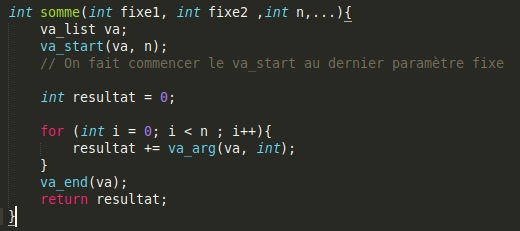
\includegraphics[scale=0.6]{fonctionParamVar}
\end{center}
\end{itemize}

\subsection{Pointeur de pointeur}
\begin{itemize}
\item Pointeur de pointeur : int a = 1; int *ptr = \&a; int **pp = \&ptr;
\item \href{https://stackoverflow.com/questions/5580761/why-use-double-pointer-or-why-use-pointers-to-pointers}{\textit{lien internet : }utilisation pointeur de pointeur}
\item Si pp est un pointeur de pointeur pointant sur le pointeur ptr. On initialise cette variable : int **pp = \&ptr; Ainsi *pp correspond à la valeur de ptr qui est l'adresse de la variable pointée par celui-ci. Via pp, on accède à la valeur cette variable avec **pp.
\end{itemize}

\subsection{Pointeur de char}
\begin{itemize}
\item Pour déclarer un tableau de char modifiable : char tab[] = "abc"
\item En déclarant le pointeur de char : char *p = "abc" il n'est plus possible de modifier le string "abc".
\item Pour printf le pointeur p : \textit{printf("\%s",p);}
\item Dans malloc il y a déjà un free(). Donc pour changer le mot contenu dans un char * via une fonction dans laquelle il est un argument on peut faire de la façon suivante:
\newline void changerMot(char **pp, char *mot)\{
\newline *p = malloc(sizeof(mot)) \textit{permet de free() le pointeur qui a la chaine de caractère}
\newline *p = mot; \}
\newline Pour utiliser cette fonction : \textit{changerMot(\&tableauDeChar, "unMot")}
\end{itemize}

\subsection{Les listes chaînées}
\begin{itemize}
\item \href{https://openclassrooms.com/fr/courses/19980-apprenez-a-programmer-en-c/19733-les-listes-chainees}{lien  tutorial 1 sur openclassroom}
\item \href{run:../Test C/}{programme liste\textunderscore chainee.c}
\item Une liste chaînée est un moyen d'organiser une série de données en mémoire. Cela consiste à assembler des structures en les liant entre elles à l'aide de pointeurs
\item La structure est organisée de la manière suivante :
\newline 1. Elément stocké 2. Un poiteur pointant sur la case d'après
\item La liste est dite chainée car elle constitue une chaîne de pointeur qui relie les différents éléments.
\item A la différence des tableaux, les éléments dans cette liste chaînées ne se suivent pas dans la mémoire. Tous ces éléments sont donc stockés dans différents endroit de la mémoire d'où la nécessité des pointeurs.
\item Comment construire une chaîne de caractère ? On va d'abord créer une structure qui va constituer le schéma de chaque maillon dans cette chaîne. Il faut donc initialiser une structure. Considérons une liste chaînée d'entiers.
\item Initialisation de la structure Element : 
\newline \textit{typedef struct Element Element;}
\newline \textit{struct Element \{ int nombre; Element *suivant;\};}
\newline Ce schéma de maillon constitue va permettre de créer une liste dite "simplement chaînée" puisqu'on ne peut connaître que le maillon suivant. Lorsqu'une structure prend en compte le maillon précédent on parle de liste "doublement chaînée". Cela dit, l'utilisation de ce type de chaîne devient alors plus complexe.
\item Il faut en plus créer une structure qui va permettre de contrôler l'ensemble de la liste chaînée. Elle contient ainsi le premier élément de la liste chaînée. On peut aussi stocker la taille de la liste chaînée.
\item Initialisation de la structure Liste :
\newline \textit{typedef struct Liste Liste;}
\newline \textit{struct Liste \{unsigned int taille; Element *premier;\};}
\item Il faut aussi penser au dernier élément de la liste. Comment faire pour savoir que c'est le dernier ? La solution la plus efficace est de faire pointer le pointeur du dernier élément sur \textit{NULL}.
\begin{center}
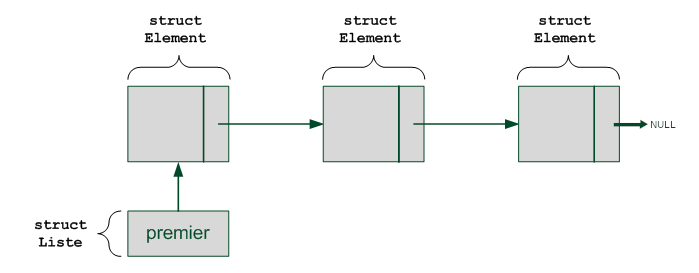
\includegraphics[scale=2]{schema_liste_chainee}
\end{center}
\item Il faut alors créer des fonctions pour manipuler la liste chaînée. Par exemple nous pouvons :
\begin{enumerate}
\item initialiser la liste (on pourrait aussi utiliser : \textit{void initialisation (Liste *liste)})
\item ajouter des éléments
\item supprimer des éléments
\item afficher les éléments de la liste chaînée
\item supprimer la liste chaînée
\newline
 \begin{minipage}{\linewidth}
  \begin{figure}[H]
  \centering
    \subfloat[Liste *initialisation()]{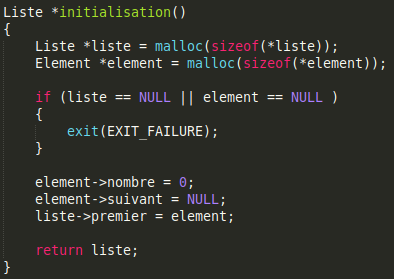
\includegraphics[scale=0.4]{initialisation}}\hspace{1cm}
    \subfloat[void insertion(Liste*, int)]{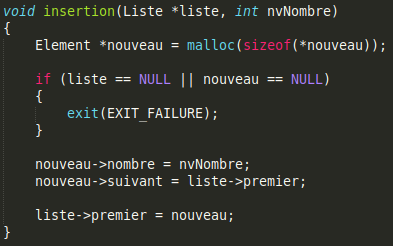
\includegraphics[scale=0.4]{insertion}}
  \end{figure}
  \begin{figure}[H]
  \centering
    \subfloat[void suppression(Liste*)]{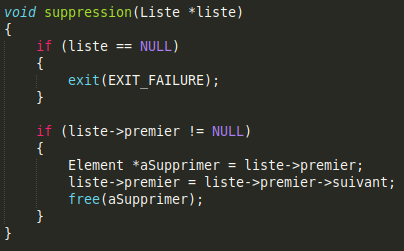
\includegraphics[scale=0.4]{suppression}}\hspace{1cm}
    \subfloat[void afficherliste(List*)]{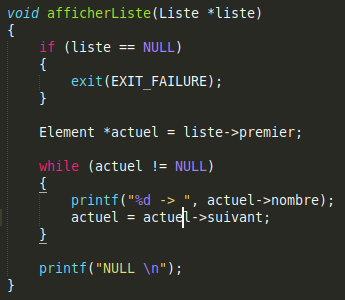
\includegraphics[scale=0.4]{afficherListe}}
  \end{figure}
  \end{minipage}
\end{enumerate}

\end{itemize}


\subsection{Récursivité}
\begin{itemize}
\item \href{https://franckh.developpez.com/tutoriels/c-ansi/recursivite/}{Lien tutorial récursivité}
\item \href{run:../Test C/}{fichier programme récursivité}
\item Exemple de fonction récursive avec la fonction \textit{factorielle} :
\item \textit{unsigned int factorielle(int n)\{ }
\newline \textit{if (n == 1) return 1L;}
\newline \textit{return n * factorielle(n-1)\}}
\item Les appels des fonctions récursives sont ainsi empilés jusqu'à la condition de sortie ici \textit{n == 1}.
\begin{center}
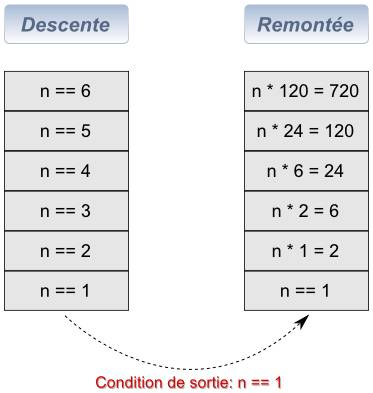
\includegraphics[scale=0.5]{piles_de_recursivite}
\end{center}
\item Cette méthode est appelée \textit{récursivité normale}. Cette méthode est efficace mais peut poser problème si la récursivité est trop longue. En effet, il risque d'y avoir une explosition de lq pile ce qui entraînerait un plantage du programme. C'est pour cela que nous allons voir une autre méthode : \textit{la récursivité terminale}
\item Les fonctions récursives normales ont un argument en plus. Il n'y a alors qu'une descente de la pile et donne le résultat final à la fin.
\newline \textit{unsigned long factoriel \textunderscore terminal (int n, unsigned long result)\{}
\newline \textit{   if (n == 1) return result;}
\newline \textit{   else if (n == 0) return 1L;}
\newline \textit{   return factoriel\textunderscore terminal (n - 1, n * result);\}}

\end{itemize}


\end{document}